\documentclass[10pt,sans,english,compress,xcolor=dvipsnames]{beamer}
\author[Lily ]{ Dr Lily Asquith (Lily, she/her)}

\usetheme{Szeged}
%\defbeamertemplateparent{enumerate items}{enumerate item,enumerate subitem,enumerate subsubitem,enumerate mini template}
\definecolor{titcol}{RGB}{16,78,100} 
\setbeamercolor{frametitle}{fg=titcol,bg=White}
\useoutertheme{miniframes} 
\useinnertheme{rectangles}

\usepackage{pifont}
\newcommand{\tick}{\textcolor{grn}{\ding{52} } }
\newcommand{\nope}{\textcolor{red}{\ding{54} } }


\usepackage{soul}
\usepackage{cancel}

\usepackage[most]{tcolorbox}
\definecolor{LilyBlack}{rgb}{0.05,0.1,0.3} % UBC Blue (primary)
\usecolortheme[named=LilyBlack]{structure}

\usepackage{booktabs}
\usepackage{tabularx}
%\usepackage{tikz}
%\def\checkmark{\tikz\fill[scale=0.4](0,.35) -- (.25,0) -- (1,.7) -- (.25,.15) -- cycle;}

\usepackage{physics}

\usepackage{xparse}

\setbeamertemplate{footline}{%
  \leavevmode%
  \hbox{\begin{beamercolorbox}[wd=.5\paperwidth,ht=2.5ex,dp=1.125ex,leftskip=.3cm plus1fill,rightskip=.3cm]{author in head/foot}%
    \usebeamerfont{author in head/foot}\insertshortauthor
  \end{beamercolorbox}%
  \begin{beamercolorbox}[wd=.5\paperwidth,ht=2.5ex,dp=1.125ex,leftskip=.3cm,rightskip=.3cm plus1fil]{title in head/foot}%
    \usebeamerfont{title in head/foot}\insertshorttitle\hfill\insertframenumber\,/\,\inserttotalframenumber
  \end{beamercolorbox}}%
  \vskip0pt%
}

\DeclareMathSizes{10}{10}{6}{4} % this one
%\DeclareMathSizes{10.95}{10}{6}{4}   % For size 10 text

\newcommand*\ColorBox[3][black]{%
  \makebox[2em][c]{%
    \setlength\fboxsep{-.5\fboxrule}%
    \raisebox{\dimexpr-#3em+.5ex}{%
      \fcolorbox{#1}{#2}{%
        \rule{0pt}{\dimexpr#3em*2}%
        \rule{\dimexpr#3em*2}{0pt}%
      }%
    }%
  }%
}

\usepackage{hyperref}
\hypersetup{
    colorlinks=true,
    linkcolor=blue,
    filecolor=magenta,      
    urlcolor=blue,
    pdftitle={Overleaf Example},
    pdfpagemode=FullScreen,
    }

\urlstyle{same}

% this part excludes specified frames from counters in navigation bar
\makeatletter
\let\beamer@writeslidentry@miniframeson=\beamer@writeslidentry
\def\beamer@writeslidentry@miniframesoff{%
  \expandafter\beamer@ifempty\expandafter{\beamer@framestartpage}{}% does not happen normally
  {%else
    % removed \addtocontents commands
    \clearpage\beamer@notesactions%
  }
}
\newcommand*{\miniframeson}{\let\beamer@writeslidentry=\beamer@writeslidentry@miniframeson}
\newcommand*{\miniframesoff}{\let\beamer@writeslidentry=\beamer@writeslidentry@miniframesoff}
\makeatother


\makeatletter
\newcommand\notsotiny{\@setfontsize\notsotiny{6.5}{7.5}}
\makeatother




\usepackage{multicol}
\usepackage{sansmath}
\usepackage{minted}
\definecolor{LightGray}{gray}{0.95}


\title[RVs and Data]{Random Variables, Describing Data}
\date{}
\titlegraphic{
%\center

\includegraphics[scale=0.15]{sussex-logo}
}


\begin{document}


\newcommand\info{\mathcal{J}_{\theta}}
\newcommand\loglike{\ln{ \mathcal{L}_{\theta}} }
\newcommand\like{\mathcal{L}_{\theta} }

\newcommand\thetahat{\hat{ \theta }  }

\definecolor{grn}{RGB}{0,128,0} 
\newcommand{\gbl}[1]{\textcolor{grn}{#1}}

\definecolor{wh}{rgb}{0.95, 0.95, 0.96}
\newcommand{\wht}[1]{\textcolor{wh}{#1}}

%\newcommand{\inprob}{\overset{p}{\to}}

\newcommand{\boo}[1]{\textbf{\textcolor{red}{#1}}}

\newcommand{\covmat}{\mathbf{\textcolor{magenta}{\Sigma}} }


\definecolor{purr}{RGB}{128,0,128} 
\newcommand{\purp}[1]{\textcolor{purr}{#1}}

\newcommand{\magt}[1]{\textbf{\textcolor{magenta}{#1}}}
 \newcommand{\magtn}[1]{\textcolor{magenta}{#1}}
 
%\definecolor{bbl}{RGB}{128,0,128} 
\newcommand{\bbl}[1]{\textcolor{blue}{#1}}

\newcommand{\rbl}[1]{\textcolor{red}{#1}}

\definecolor{dblu}{RGB}{37,150,190} 
\newcommand{\blu}[1]{\textcolor{dblu}{#1} }

\definecolor{dor}{RGB}{255,40,0} 
\newcommand{\dor}[1]{\textcolor{dor}{#1} }

\definecolor{darkgreen}{RGB}{46,139,87} 
\newcommand{\dgreen}[1]{\textbf{\textcolor{darkgreen}{#1}} }
%\newcommand{\gbl}[1]{\textcolor{darkgreen}{#1}}

\definecolor{lgray}{RGB}{222,222,222} 

\definecolor{lyellow}{RGB}{255,255,224} 

\newcommand{\E}[1]{\mathbf{E}_{#1}}
%
\newcommand{\rvX}[1]{X_{(#1)} } 

\newcommand{\rvY}[1]{Y_{(#1)} }

\newcommand{\rvx}[1]{x_{(#1)} } 

\newcommand{\rvy}[1]{y_{(#1)} }



\newcommand{\red}[1]{\textcolor{red}{#1} }

\newcommand{\bluedots}{\blu{\ldots} }

\newcommand{\dordots}{\dor{\ldots} }


\newcommand{\where}{\dgreen{\;where\;} }


\newcommand{\pand}{\dgreen{\;and\;} }
\newcommand{\por}{\dgreen{\;or\;} }

\newcommand{\sumN}{ \sum\limits_{\blu{i}}^{\blu{N}} }

\newcommand{\sumZ}{ \sum\limits_{\dor{j}}^{\dor{Z}} }

\newcommand{\Expec}[1]{ \mathbb{E}[#1] }


\newcommand{\Xfj}[1]{ X_{ \dor{#1} } }

\newcommand{\xfi}[1]{ x_{ \blu{#1} } }

\newcommand{\Xij}[2]{ X_{\mage{#1},\blu{#2} }}

\newcommand{\sumxi}{ \sumN \xfi{i} }

\newcommand{\sumXj}{ \sumZ \Xfj{j} }

\newcommand{\sumZa}[1]{ \sumZ {#1}_{ \dor{j} } }

\newcommand{\sumZab}[2]{ \sumZ {#1}_{ \dor{j} }\, {#2}_{ \dor{j} } }

\newcommand{\sumNab}[2]{ \sumN {#1}_{ \blu{i} }\, {#2}_{ \blu{i} } }

\newcommand{\vecxi }{ [ \xfi{1} \xfi{2}, \bluedots, \xfi{N} ] }

\newcommand{\vecXj }{ [ \Xfj{1} \Xfj{2}, \bluedots, \Xfj{Z} ] }

\newcommand{\vecXij }{ [ \Xij{1}{1} \Xij{1}{2}, \bluedots, \Xij{1}{N_1} ],\, [ \Xij{2}{1} \Xij{2}{2}, \bluedots, \Xij{2}{N_2} ],\, \dordots,\,[ \Xij{Z}{1} \Xij{Z}{2}, \bluedots, \Xij{Z}{N_Z} ] }

% definitions

\newcommand{\overNblack}{ \dfrac{1}{N} }
\newcommand{\overN}{ \dfrac{1}{ \blu{N} } }

\newcommand{\defmean }{ \overline{x} = \overN \sumN \xfi{i} }

\newcommand{\meanx }{ \overline{x} }
\newcommand{\meansqx }{ \overline{x^2} }
\newcommand{\sqmeanx }{ \overline{x}^2 }
\newcommand{\devsq}{ (\xfi{i} - \meanx)^2 }

%\newcommand{\var }[1]{ \mathcal{V}_{#1} }
\newcommand{\defvar }{ \var{x} = \overN \sumN \devsq }
\newcommand{\defvarshort }{ \var{x} = \meansqx - \sqmeanx }

\newcommand{\defstd }{ s_x = \sqrt{ \var{x} }  }

\newcommand{\defwmean }{ \overline{X} = \dfrac{ \sumZab{w}{X} }{ \sumZa{w} } }  

\newcommand{\defw }{ w_{\dor{j}} = \dfrac{1}{ \var{\Xfj{j} } } }

\renewcommand{\boo}[1]{\textbf{\textcolor{red}{#1}}}


\begin{frame}
\titlepage
\end{frame} 

\section*{Preamble}

\begin{frame}[fragile]{News}

%Canvas announcements digest:\\
\begin{itemize}
\item Changing lecture/workshop times non-trivial and unlikely to happen.\\
\item There is a zoom link for every lecture and workshop. Not full hybrid.\\
\item Workshop problems are on canvas week 2 page.\\
\item Assignment 1 is on canvas Assignment \& Guidance page\.\
\item I made a slack channel for those who want it.\\
\item I made an anonymous google form for PIPS times.\\
\item Python/marimo  issues: please ask your fellow students.\\
\item Attendance etc, please email: fosem-info@sussex.ac.uk \\
\end{itemize}




\end{frame} 


% python
\begin{frame}[fragile]{Following with Python}

Install marimo as per instructions on canvas: Resources \& Prerequisites\\[1ex]

\begin{minted}[bgcolor=LightGray]{bash}
pip install marimo
\end{minted}

Download the notebook from the canvas page for this week's material: \dgreen{RandomVariables.py} \\[1ex]

\begin{minted}[bgcolor=LightGray]{bash}
marimo edit RandomVariables.py
\end{minted}

\end{frame} 


\begin{frame}{Data}
\large
\begin{itemize}
\item Random Variables\\[1ex]
\item Mean \& Expected Value\\[1ex]
\item Variance \& Standard Deviation\\[1ex]
\item Weighted Mean \& Variance\\[1ex]
\item Other Definitions\\[1ex]
\end{itemize}

\end{frame} 

\section*{Random Variables }


\begin{frame}{What is a Random Variable?}

A \boo{Random Variable (RV)} is a \textbf{function} that maps events to real numbers. $X(A_i) = x_i$ for all $A_i \in S $\\[1ex]

\begin{center}
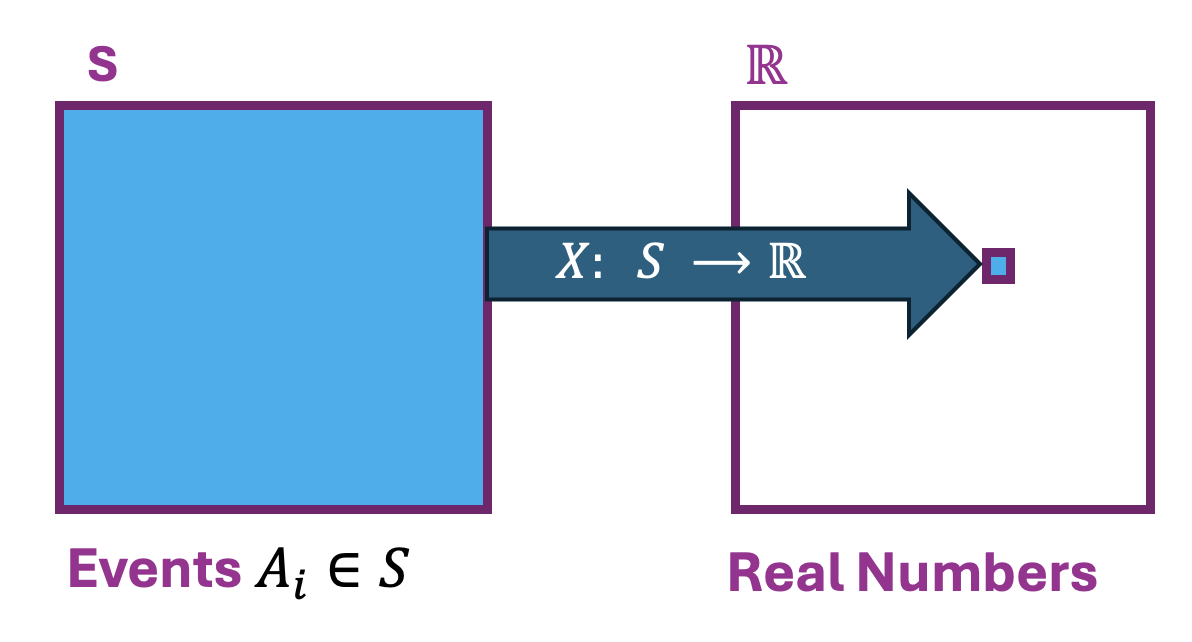
\includegraphics[scale=0.3]{rv1}
\end{center}


$X$ is the RV: a function\\[1ex]
$A_i$ is an event in the sample space S of all possible events. \\[1ex]
$x_i$ is the value  corresponding to this event, according to $X$.\\[1ex]

\end{frame} 


\begin{frame}{Random Variables: Example of Height }

The \boo{RV} $X$ is the function that turns the abstract concept of height into a number and unit.\\[1ex]

$X(\mathsf{abstract\; concept\; of\; Lily's\; height}) = 1.71\mathsf{\,m}$\\[1ex]

$X(A_i) = x_i$ for all $A_i \in S$\\[1ex]

$A_i$ is a height from the sample space S of all possible heights. \\[1ex]
$x_i$ is the value corresponding to this height, according to $X$.\\[1ex]

\end{frame} 





\begin{frame}{
\only<1>{General Notation used by me in this module}
\only<2>{General Notation: RVs}
\only<3>{General Notation: Datasets}
\only<4>{General Notation: Measurements}
}

$Z$: the number of Random Variables under consideration\\[2ex]

\textbf<2>{$X= \{X_{(1)}, X_{(2)}, ..., X_{(Z)} \}$  the $Z$ Random Variables}.\\[2ex]

\textbf<3>{$x = \{x_{(1)}, x_{(2)}, ..., x_{(Z)}\}$  the $Z$ Datasets}\\[2ex]

\textbf<4>{$x_{(j)}= \{x_{j,1}, x_{j,2}, ..., x_{j,N}\} $ is a Dataset of $N$ Measurements}\\[2ex]

\only<1>
{
\blu{If we have one RV, I will say that the Dataset is one-dimensional (1D) and $X$ is the single RV. Almost all examples in this topic are 1D.}\\[1ex]
}

\only<2>{
\blu{
Note that the RVs are denoted by the symbol $X$ no matter whether there is one or fifty of them. I do not use the vector notation eg  $\vec{X}$. Assume all $X$ are sets of $Z$ $X_{(j)}$s.}\\[1ex]
}

\only<3>{
\small
\blu{
Each dataset is denoted $x_{(j)}$ where the subscript $(j)$ identifies which RV the measurements are for. The brackets around the datasets' RV identifiers are there to remind us that $x_{(j)}$ is not a number but a set of them. This is needed because when we see $x_j$ our brains say `number'.}
}

\only<4>{
\blu{I like to use the identifiers $i,... N$ for measurements, and $j,... Z$ for RVs (or sometimes for experiments - more later).}
}

\end{frame} 




\begin{frame}{Notation Example}

Say we are measuring the heights and weights of a sample of 10 people:\\[1ex]

$Z = 2$\\

$X = \{H,W\}$  are the RVs:  $H$ is height and $W$ is weight.\\

$x = \{h,w\}$  are the datasets: $h$ are the measured height values and $w$ are the measured weight values.\\

$h = \{h_1, h_2, ..., h_{10}\} $ is a dataset of the $N=10$ height measurements $h_i$.\\

\blu{Notice that $x$ is a matrix with 2 rows and 10 columns}\\

\end{frame} 


%\begin{frame}{When There is One RV}
%
%Almost everything in these slides can be explained completely with one RV, and so is.\\[1ex]
%
%If we have one RV, the Dataset is one-dimensional (1D)\\[1ex]
%
%I will say this, and that $X=X_{(1)}$, then continue to use $X$ as my one RV, and $x=x_{(1)}$ as my 1D dataset.\\[1ex]
%
%This ups the chance of confusion but massively improves the readability of formulae.\\[1ex]
%
%\end{frame} 




\begin{frame}[fragile]{Continuous RVs}

A  \boo{Continuous Random Variable (CRV)} is one for which the measurements can take any value (such as height and weight).\\[2ex]
Note that in the real world, measurements always have a finite precision. So the measurements $x$ of a CRV $X$ will not strictly be continuous.\\[2ex]
What is true in the real world is also in true in your computer. The precision with which python generates CRVs on my machine is 'float64': precision 15.\\[2ex]
\blu{A continuous RV is still continuous even though its measurements cannot be.}\\

%\vspace{1cm}
%\begin{minted}[bgcolor=LightGray]{python}
%# Draw 10 crvs in range (0,100) 
%crvs_x = random.uniform(0,100,10)  
%\end{minted}

\end{frame} 


\begin{frame}[fragile]{Discrete RVs}

A  \boo{Discrete Random Variable (DRV)} is one for which the measurements can only take certain values (such as a roll of dice).\\[2ex]
Discrete RVs don't have to be integers, but they do have to be countable.\\[2ex]

\blu{For example, the probability of dice rolls (any number of dice) are not integers but are Discrete. As I increase the number of dice and/or rolls, I can generate lots of probability values from the original set, but there will always be real numbers I cannot generate (gaps).} \\
 
%\vspace{1cm}
%\begin{minted}[bgcolor=LightGray]{python}
%# Draw 10 integer rvs in range (0,100) from randint
%drvs_x = random.randint(0,100,10)
%\end{minted}

\end{frame} 

\begin{frame}{Distribution Functions}
A \boo{Distribution Function} $f(X;\theta)$ is a theoretical object that describes the True Distribution of the RVs $X$. \\[1ex]
\blu{Recall, the RV is a function that returns a real value. So the distribution of $X$ is the distribution of all the possible values that could be returned by $X$.}\\[1ex]
The true parameters are denoted by $\theta$.\\[1ex]
For example, a straight line:\\[1ex]
 $f(X;m,c) =mX+c$ is written\\[1ex]
 $f(X;\theta) =\theta_1 X+ \theta_0$\\[2ex]
% \blu{There is no obvious benefit to using this (hideous?) notation so far, but in the case of many RVs or many parameters things quickly get very messy if we don't fold up our RVs and parameters neatly.}
%\textbf{Why not just use $X, Y$ for RVs and $m,c$ for parameters?!} It gets messy quickly with more than two. It is better this way.\\
If there is only one parameter, and $f(X;\theta)$ is a familiar function such as exp or norm (later!) then we often use a symbol for the parameter to reflect that such as $\mu$ or $\lambda$.\\
\end{frame}

% Normalisation
\begin{frame}{Distribution Function (DF) as Probability (PDF)}
Any DF of a continuous RV can be turned into a Probability DF. For example: \\[1ex]
\boo{ $f(X;\theta) = x^3$ is a function}\\[1ex]
\begin{itemize}
\item[1] Write $f(X;\theta) = A x^3$\\[1ex]
\item[2] Specify the `range', for example $X:[0,1]$\\[1ex]
\item[3] Set integral to one: $\int\limits_0^1   A x^3 dx =1$\\[1ex]
\item[4] Solve for A:  $A \dfrac{1}{4} =1 \therefore A= 4 $\\[2ex]
\end{itemize} 
\boo{$f_X = 4x^3$ for $0\leq x \leq 1$ is a valid PDF}. Total Probability (Integral) is 1.\\[1ex]

\end{frame} 


\begin{frame}{The True Distribution}
The 1D dataset $x=x_{(1)}$ in this histogram ($N=100$ measurements) has a familiar shape. Looks like exponential decay! (\blu{I cheated - it is fake data})\\[1ex]
Drawing  the exponential function over the top confirms it is similar. \\
\center
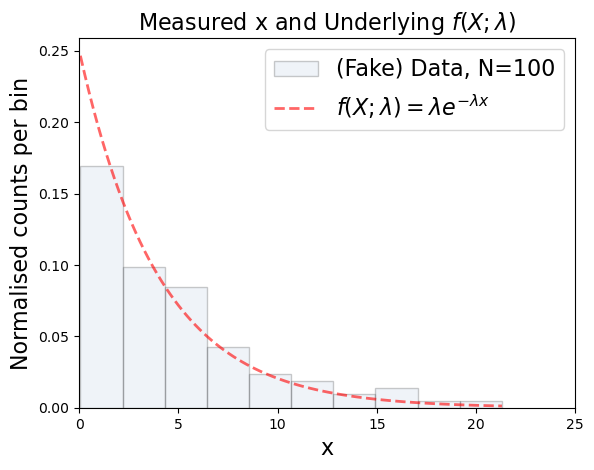
\includegraphics[scale=0.38]{PLOTDAT1-HistAndFunc_Expo_N100_Lambda0.25.png}

%\small
%\textcolor{red}{I know you have questions. I promise we will answer these in time.}
\end{frame}

\begin{frame}{Distribution Functions}
If I collect (okay, fake) more data ($N=1000$), the agreement looks more convincing. \\[1ex]
\center
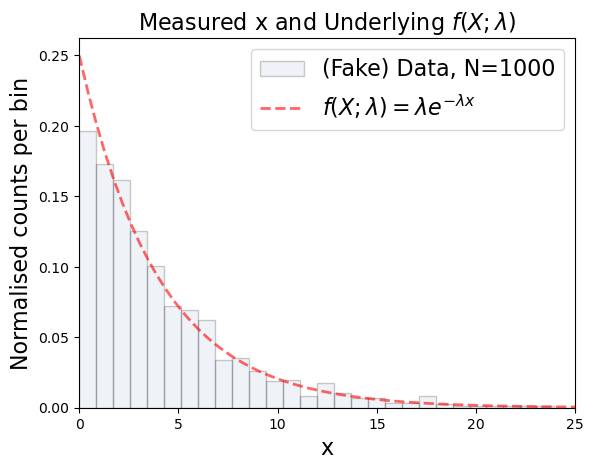
\includegraphics[scale=0.38]{PLOTDAT1-HistAndFunc_Expo_N1000_Lambda0.25.png}
\end{frame}

\begin{frame}{Distribution Functions}
Even more data ($N=10,000$), now they are indistinguishable by eye. \\[1ex]
\begin{center}
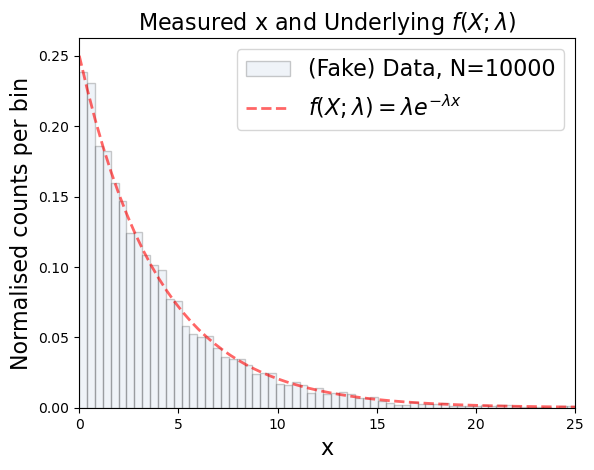
\includegraphics[scale=0.38]{PLOTDAT1-HistAndFunc_Expo_N10000_Lambda0.25.png}
\end{center}

%In the limit of infinite measurements, the $x$ distribution is the true $X$ distribution. \\[1ex]
\end{frame}


% IID
\begin{frame}{Independent \& Identically Distributed RVs}
A collection of RVS is \boo{Independent and Identically Distributed (IID)} if:\\[1ex]

\begin{itemize}
\item[1] They are all mutually independent \textbf{and}\\[1ex]
\item[2] They all have the same underlying probability distribution.\\[1ex]
\end{itemize}
\vspace{1cm}
\boo{Mutually independent RVs}: measuring any of them has no effect on the probabilities of the others.\\

\end{frame}

% IID
\begin{frame}{IID RVs Example}

The result of tossing a coin once is a RV $X_{(1)}$. It can have values $x_{(1)}=\{\mathsf{heads}, \mathsf{tails}\}$\\[1ex]
The result of tossing  the coin again is also a RV, $X_{(2)}$. The same values are possible.\\[1ex]

The result of the first toss does not have any effect on the result of the second toss. So the RVs $X_{(1)}$ and  $X_{(2)}$ are \boo{Mutually Independent}.\\[1ex]

The probability of each toss coming up heads is identical, so the RVs are \boo{Identically Distributed}. \\[1ex]
\blu{This is true even if the coin is not fair, because it is the same coin being tossed both times.}

\end{frame}



% SEC: MEAN AND EXPEC
\section*{Mean \& Expectation}


\begin{frame}[fragile]{The Mean of a Dataset}

The \boo{Mean} of a 1D dataset ($x = x_{(1)}$) is:\\[1ex]
 $\overline{x} = \dfrac{1}{N} \sum\limits_i^N x_i$, \\[1ex]

\blu{where the sum is over the $N$ measurements}\\[1ex]
%\vspace{1cm}
%\begin{minted}[bgcolor=LightGray]{python}
%# longhand
%mean_x = np.sum(crvs_x) / np.size(crvs_x) 
%# using numpy mean
%mean_x = np.mean(crvs_x) 
%\end{minted}


\end{frame}


%BINNED MEAN
\begin{frame}[fragile]{The Binned Mean}

The \boo{Binned Mean} is important in real life (\blu{why?}). It is written:\\[1ex]
 $\overline{x} = \dfrac{1}{N} \sum \limits_i^M n_i\, c[x]_{i}$ \\[1ex]

\blu{Here $n_i$  is the number of entries in bin $i$,  $c[x]_i$ is the central value of that bin, and the sum is over the $M$  bins rather than the $N$  individual values. }\\[1ex]

Note that we must still normalise using the number of measurements, $N$.\\

%\vspace{1cm}
%\begin{minted}[fontsize=\footnotesize, bgcolor=LightGray]{python}
%# The Binned mean
%# see marimo, too long for slide
%\end{minted}


\end{frame}



\begin{frame}[fragile]{The Binned Mean }
$\overline{x} = \dfrac{1}{N} \sum \limits_i^M n_i\, c[x]_{i}$ \\[1ex]
Each of the red dots is $(c[x]_{i}, n_i)$ : (bin center, bin count) \\[1ex]
 
 \center
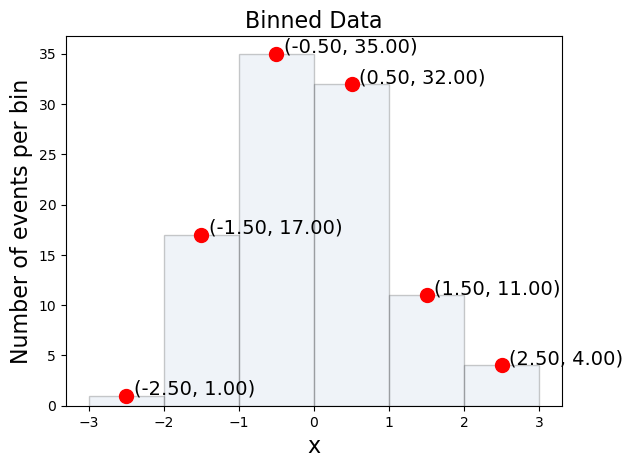
\includegraphics[scale=0.4]{PLOTDAT1-Histogram.png}

\end{frame}





\begin{frame}[fragile]{The Expected Value}

The \boo{Expected Value}* of a single RV $X=X_{(1)}$  is the \boo{True Mean}:\\[1ex]

$E[X] =  \sum\limits_i^\infty x_{i} p_i$ \blu{($X$: discrete)}\\[1ex]

 where $p_i$  is the probability of observing the measurement $x_i$. \\[1ex]

If the probabilities of the measurements are described by a \textit{Probability Density Function} $f_X$ (with integral=1), then we can write this:\\[1ex]

 $E[X] =  \int \limits_{-\infty}^{\infty} x\, f_X\, dx$ \blu{($X$:continuous)}\\[1ex] % 
\includegraphics[scale=0.15]{goldy} \\[1ex]

\textbf{Equivalent notation $E[X] \equiv \langle X\rangle \equiv \mu $.}\\[1ex]
* Also known as the Expectation or Expectation Value. \\[1ex]
\end{frame}



\begin{frame}[fragile]{Aside: The Expected Value for data }

%Notice that the Expected Value is a Weighted Mean:\\
%$E[X] =  \sum\limits_i^\infty x_{i} p_i$ \blu{($X$: discrete)}\\[1ex]

The Expected Value of a Dataset of $N$ measurements: $E[x] =  \sum\limits_i^N x_{i} p_i$.\\[1ex]

We can use this: what would you \textbf{expect} the average number of sixes to be from 100 dice rolls?\\[1ex]

Probability is flat $p_i = \dfrac{1}{6}$  and $x_{i} =1$ for a positive outcome (rolled a six)\\[1ex]

$E[x] =  \sum\limits_1^{100}  1\cdot\dfrac{1}{6} = \dfrac{100}{6} $\\[1ex]

\blu{Note that E[x] is a prediction we can only use when we are certain of the probabilities before hand.}

\end{frame}


%
%% ASIDE NORMED FX
%\begin{frame}[fragile]{Aside: Probability Density Functions}
%\small
%
%We will dedicate subtantial time to PDFs these over the next weeks. The plots included in these slides use the \texttt{scipy.stats} PDFs \texttt{expon} and \texttt{norm} which are known to occur in nature (more on that later!). \\[1ex]
%To practise with the true statistics such as E[X], you can use any function provided it is \textbf{Normalised} (integral =1) over the range you are using it.\\
%
%\begin{minted}[fontsize=\footnotesize, bgcolor=LightGray]{python}
%from scipy.stats import rv_continuous
%# normed x^3 over range 0,100
%class fx_pdf(rv_continuous):
%    def _pdf(self,x):
%        return 4e-08*x**3
%normed_fx = fx_pdf(a=0, b=100)
%expect = normed_fx.expect()                        
%var = normed_fx.var()
%\end{minted}
%\end{frame}
%To practise with the true statistics such as E[X], you can use any function provided it is \boo{Normalised}. (Kolmogorov 2: total probability is 1).
%
%A \boo{Normalised} distribution has integral =1: $\int \limits_S f_X dx= 1$ where S is the range of validity, which you can choose.\\
%
%For example $f_X = Ax^3$ $\int \limits_{0}^{1} Ax^3 dx= A\dfrac{1^4}{4}  \therefore A=4$:  $f_X = 4x^3$ is Normalised in the range $x:[0,1]$\\
%
%If you would like to do python checks on statistics such as the Expectation Value and True Variance, you can do.\\[1ex]
%


\begin{frame}[fragile]{The Expected Value and the Mean}

The \boo{Expected Value} of the RV:  $E[X] =  \sum\limits_i^\infty x_{i} p_i$, \\[1ex]
The \boo{Mean} of the Measurements:  $\overline{x} = \dfrac{1}{N} \sum\limits_i^N x_i$, \\[1ex]
Observations:\\[1ex]
\begin{itemize}
\item[1] $E[X]$ sum is to infinity: \blu{because in truth, there are $\infty$ values for $X$.}
\item[2] $E[X]$ doesn't have the $\dfrac{1}{N}$ normalisation:  \blu{the normalisation is taken care of by $p_i$.}
\item[3] $E[X]$ has $p_i$: \blu{$p_i$ is the probability of observing $x_i$.}
\end{itemize}

\end{frame}


\begin{frame}[fragile]{The Expected Value and the Mean}

Here is a plot of $N=100$ measurements (fake data again!) which appear to follow a Gaussian Distribution (I faked them, so they definitely do). The red dashed line is the true distribution $f_X$ of the RV $X$.\\[1ex]

\center
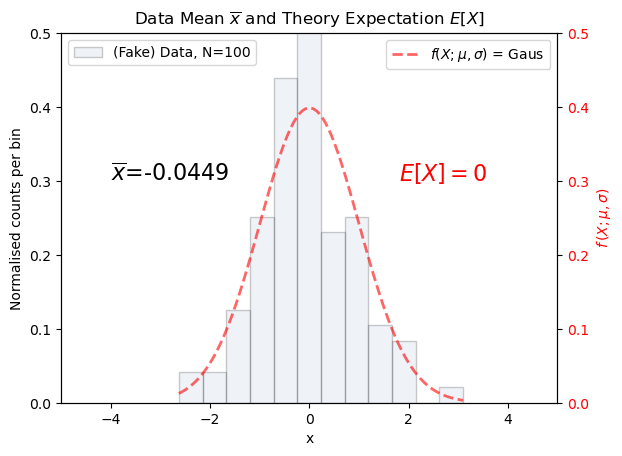
\includegraphics[scale=0.45]{PLOTDAT2-MeanAndExpec_Norm_Mu0_Sigma1_N100.png}

\end{frame}


\begin{frame}[fragile]{The Expected Value and the Mean}
Take more data: $N=1000$ measurements. The mean has changed, but E[X] has not. It is the True Mean.\\[1ex]

\center
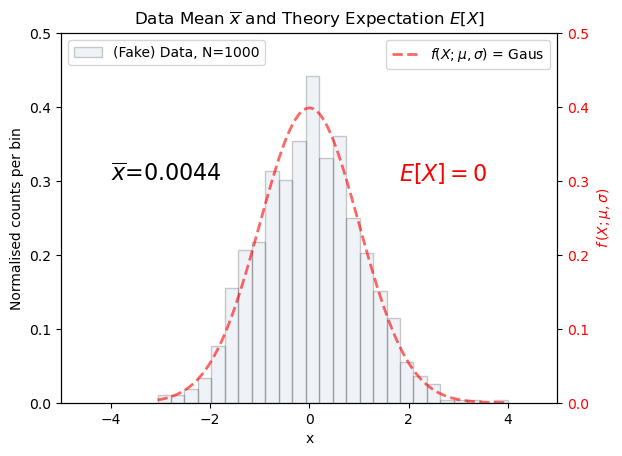
\includegraphics[scale=0.45]{PLOTDAT2-MeanAndExpec_Norm_Mu0_Sigma1_N1000.png}

\end{frame}

\begin{frame}[fragile]{The Expected Value and the Mean}

Now $N=10,000$ measurements. Notice $\overline{x}$ has moved away from $E[X]$ - that can happen.\\[1ex]

\center
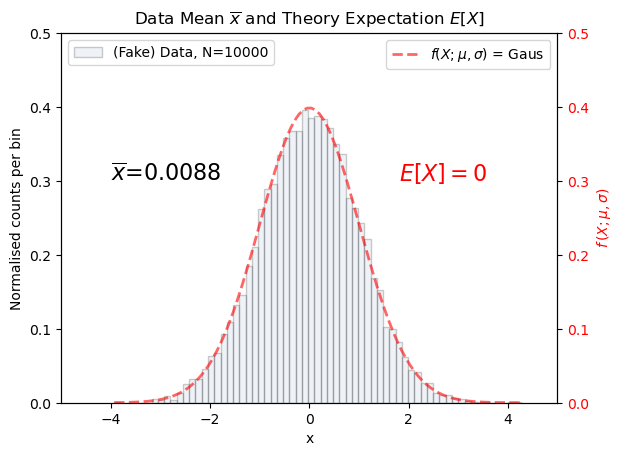
\includegraphics[scale=0.45]{PLOTDAT2-MeanAndExpec_Norm_Mu0_Sigma1_N10000.png}

\end{frame}


\begin{frame}[fragile]{The Expected Value and the Mean}
Now $N=100,000$ measurements. \boo{In the limit  $ N\rightarrow \infty$, $\overline{x} \rightarrow E[X] $} \\[1ex]
\center
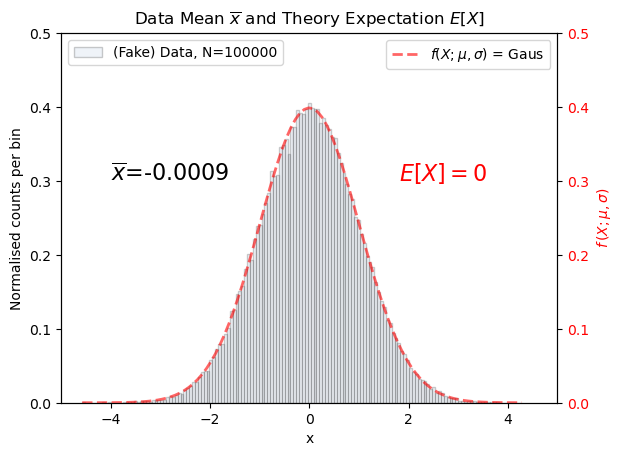
\includegraphics[scale=0.45]{PLOTDAT2-MeanAndExpec_Norm_Mu0_Sigma1_N100000.png}

\end{frame}
%
%
\begin{frame}[fragile]{Expected Value Algebra}
For RVs $A,B$: \\[2ex]
Expectation values add: $E[A+B] = E[A] + E[B] $\\[2ex]
They do not generally multiply: $E[AB] \neq E[A]E[B] $\\[2ex]
But, \textbf{if A and B are independent, they do multiply}:\\[1ex]
 \boo{$E[AB] = E[A]E[B]$ for A, B independent.}\\[2ex]

Recall: $E[X] =  \int\limits_{-\infty}^\infty x\,f_X\, dx$ \\[1ex]
\blu{If we can write $f_{XY} =f_{X}f_{Y}$, then $X,Y$ are independent.}\\[1ex]

$E[ E[A] ] = E[A]$: the expectation is a value, and the expectation of a value is just the value.\\[1ex]
\end{frame}


 %SEC: VAR
\section*{Variance \& Standard Deviation}

\begin{frame}[fragile]{Variance}
The \boo{Variance} of a set of 1D measurements $x$ is:\\[1ex]
$V[x] = \dfrac{1}{N}\sum\limits_i^N (x_i-\overline{x})^2$\\[3ex]

%\begin{minted}[fontsize=\small, bgcolor=LightGray]{python}
%# longhand
%var_x = np.sum((crvs_x-np.mean(crvs_x))**2) / np.size(crvs_x) 
%# using numpy var
%var_x = np.var(crvs_x) 
%\end{minted}

This can equivalently be written:\\[1ex]
$V[x] = \overline{x^2} - \overline{x}^2$\\[3ex]

\blu{See if you can prove these are equivalent - I will show this some time soon.}\\[1ex]

The \boo{Standard Deviation} is just the square root of the variance:
$\sigma^2_x =V[x]$ \\[1ex]

\end{frame}

\begin{frame}[fragile]{True Variance}
The \boo{True Variance} of a RV $X$ is:\\[1ex]
$V[X] = E[\,X-E[X]\,]^2$ \\[1ex]
\blu{Equivalent in mixed notation $V[X] = E[X-\mu]^2$ }\\[1ex]


This can equivalently be written:\\[1ex]
\boo{$V[X] = E[X^2] - E^2[X]$}\\[1ex] 
\blu{Equivalent in mixed notation $V[X] = E[X^2] -\mu^2$ }\\[1ex]

I think this second form is the most useful formula from this whole week.\\[1ex]

\end{frame}


\begin{frame}[fragile]{Variance is a measure of spread}
Variance: amount of spread about the mean value.\\[1ex]
Easiest to see this using this form: $V[x] = \dfrac{1}{N}\sum\limits_i^N (x_i-\overline{x})^2$.\\[1ex]
%The \boo{True Variance} of a RV $X$ is $V[X] = E[X^2] - E^2[X]$\\[1ex]
%The \boo{Sample Variance} of the dataset is  $V[x] = \overline{x^2} - \overline{x}^2$\\[1ex]

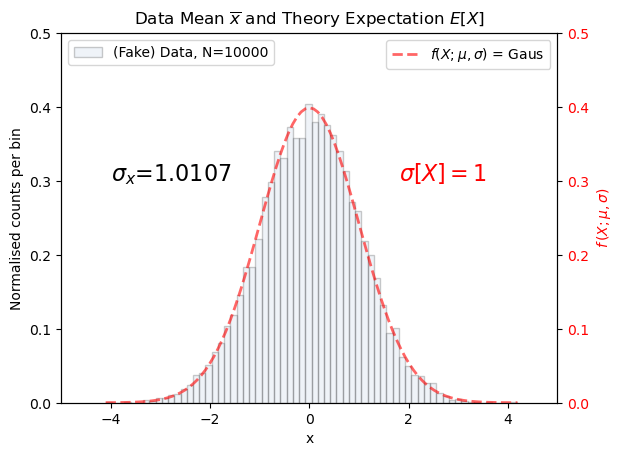
\includegraphics[scale=0.3]{PLOTDAT2-Sigma_Norm_Mu0_Sigma1_N10000.png}
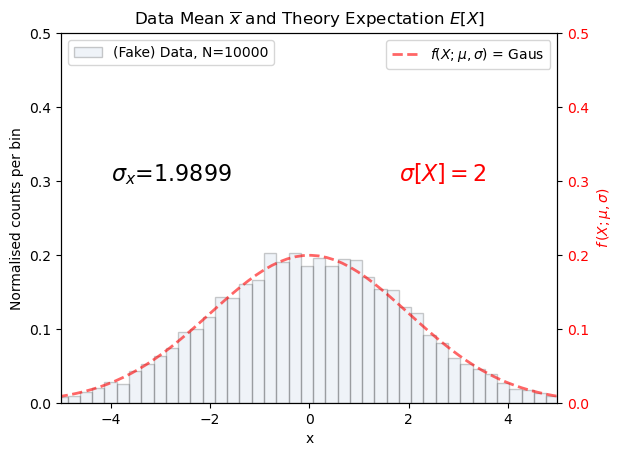
\includegraphics[scale=0.3]{PLOTDAT2-Sigma_Norm_Mu0_Sigma2_N10000.png}

It is the \boo{Standard Deviation} $\sigma_x = \sqrt{V[x]}$ that we use as our \textbf{Statistical Uncertainty} when quoting the mean of the data as $\overline{x} \pm \sigma$.\\
\end{frame}




\begin{frame}[fragile]{Aside: Unbiased Variance}
The \boo{Unbiased Variance} of a dataset of 1D measurements $x$ is:\\[1ex]
$V[x] = \dfrac{1}{N-1}\sum\limits_i^N (x_i-\overline{x})^2$\\[1ex]


\blu{This has a larger normalisation factor, and we shall see later that this takes care of the problem with calculating the variance from finite-sized dataset. I have provided a (very long) proof of this in an example attached to a later topic Introduction to Estimators.}\\[1ex]

Put a pin in this for later!\\

\end{frame}

%\begin{frame}[fragile]{Aside: Standard Deviation}
%
%The \boo{Standard Deviation} is just the square root of the variance:\\[1ex]
%
%$\sigma^2_x =V[x]$\\[1ex]
%
%It is the Standard Deviation that we use as out \boo{Statistical Uncertainty}.
%\end{frame}


 %SEC: WEIGHTED
\section*{Weighted Mean \& Variance}


\begin{frame}[fragile]{Combining Datasets}

So far we have only considered the mean and variance for a single dataset. In real life people collect many datasets of differing size and quality that are in essence measuring the same RV.\\[1ex]

To combine these datasets we want to factor in their size and quality, rather than just throw all the measurements into a single uber dataset. To do this we use \boo{Weights}.\\[1ex]

The \boo{Weighted Mean} is  $\overline{x}_w = \dfrac{\sum\limits_j^Z x_{(j)} w_j}{\sum\limits_j^Z w_j }$, where $w_j = \dfrac{1}{V[x_{(j)}]}$\\[1ex]



\end{frame}


\begin{frame}[fragile]{The Weighted Mean}

The \boo{Weighted Mean} is  $\overline{x}_w = \dfrac{\sum\limits_j^Z x_{(j)} w_j}{\sum\limits_j^Z w_j }$, where $w_j = \dfrac{1}{V[x_{(j)}]}$\\[1ex]

Note that the sum is over the $Z$ datasets, so the calculation is iterative. First find the mean and variance of each dataset (the variance is needed for the weight) then combine them.\\[1ex]

\blu{The variance on the weighted mean is no fun at this stage. We will soon see that it can be expressed very simply.}

%Spoiler: we will see later that the variance of a sum is equal to the sum of the variances.\\
%
%$V[\overline{x_w}] = \dfrac{1}{N}\,V[x_i}]  $.\\[1ex]
%
%There are many, many approaches to calculating the variance on the weighted mean. The example I give here is a good e 

%\begin{minted}[fontsize=\footnotesize, bgcolor=LightGray]{python}
%# 2 rows, each with 10 measurements
%crvs_xj = random.uniform(0,100,(2,10))
%# axis=1: dataset is row
%means_xj = np.mean( crvs_xj, axis=1)
%vars_xj = np.var( crvs_xj, axis=1)
%wmean_x = np.sum(means_xj/vars_xj)/np.sum(1/vars_xj)
%wvar_x = 1/np.sum(1/vars_xj)  
%\end{minted}

\end{frame}



 %SEC: OTHER
\section*{Other Definitions}

%median
\begin{frame}[fragile]{Definitions not used in this module}
The \boo{Median} of a dataset (or RV) is the value at which half the measurements lie at or above it.\\[1ex]

\begin{center}
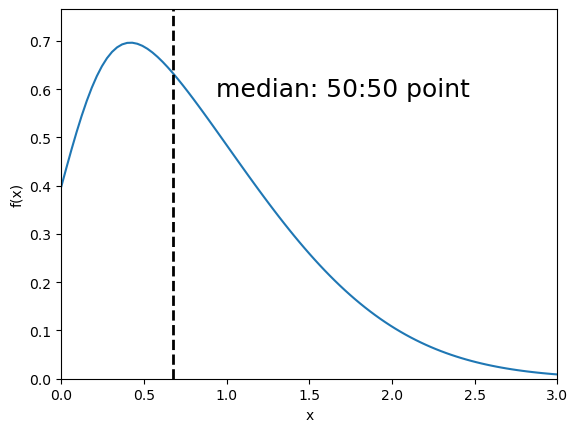
\includegraphics[scale=0.3]{PLOTDAT1-median.png}
\end{center}

%\begin{minted}[fontsize=\small, bgcolor=LightGray]{python}
%np.median(crvs_x)
%\end{minted}

\end{frame}

%mode
\begin{frame}[fragile]{Definitions not used in this module}
The \boo{Mode} of a dataset (or RV) is the most probable value.\\[1ex]

\begin{center}
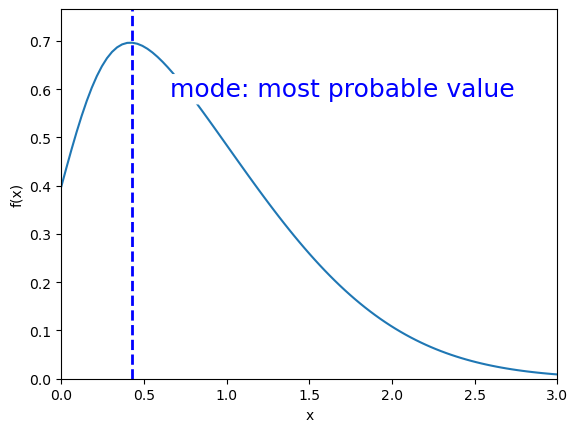
\includegraphics[scale=0.3]{PLOTDAT1-mode.png}
\end{center}

%\begin{minted}[fontsize=\small, bgcolor=LightGray]{python}
%from scipy import stats
%stats.mode(crvs_x)
%\end{minted}

\end{frame}

%rms
\begin{frame}[fragile]{Definitions not used in this module}
The \boo{RMS} (Root-Mean-Square) of a dataset is \\[2ex]

$\overline{x}_{RMS} = \left( \dfrac{1}{N} \sum\limits_i^N x^2_i \right)^{\frac{1}{2}}$\\[2ex]

The RMS is generally used in electronics and sound engineering. \\

\end{frame}


%geometric
\begin{frame}[fragile]{Definitions not used in this module}
The \boo{Geometric Mean} of a dataset  is \\[2ex]

$\overline{x}_{Geo} = \left( \prod\limits_i^N x_i \right)^{\frac{1}{N}}$\\[2ex]

The Geometric mean is sometimes used in finance. \\

\end{frame}


%fwhm
\begin{frame}[fragile]{Definitions not used in this module}
The \boo{FWHM} (Full Width at Half Max) of a dataset  is \\[1ex]

$\mathsf{FWHM} = 2\sqrt{2\ln{2}}\,\sigma \approx 2.35 \sigma$\\[1ex]

\begin{center}
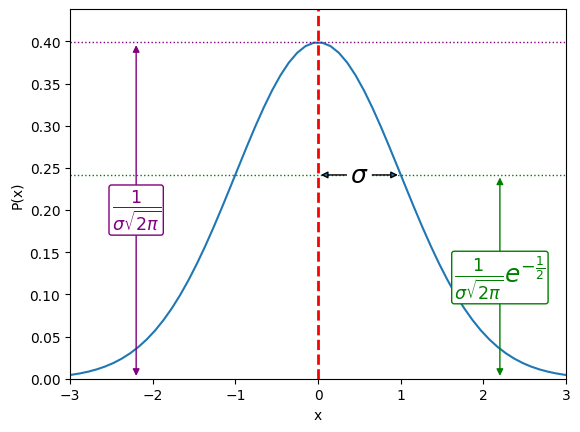
\includegraphics[scale=0.35]{PLOTDAT-MeanSigmaFWHM.png}
\end{center}

\end{frame}


%fwhm
\begin{frame}[fragile]{Definitions not used in this module}
The \boo{Skewness}  of a dataset  is $\gamma = \dfrac{1}{N} \sum\limits_0^N  \dfrac{ (x-\overline{x})^3 }{\sigma^3}$\\[2ex]

If the distribution is shifted to positive values, then the skew is positive, and vice versa.\\[1ex]

The skewness looks very similar to the variance. It is in fact the \textbf{direction of variance}. More about moments \href{https://docs.scipy.org/doc/scipy/reference/generated/scipy.stats.moment.html}{here}.\\[1ex]

\end{frame}

 %SEC: COVARIANCE
%\section*{Covariance \& Correlations}
%
%\begin{frame}{Covariance \& Correlations}
%
%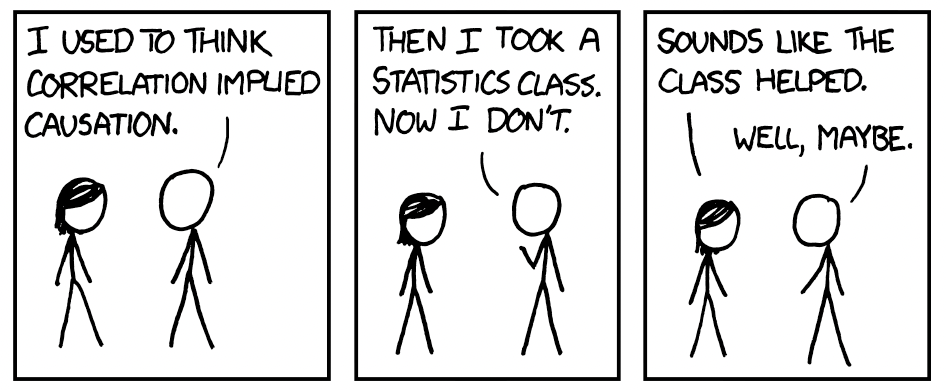
\includegraphics[scale=0.5]{xkcd-cov}
%
%\end{frame}


%\begin{frame}[fragile]{Covariance}
%
%Recall the \boo{Variance} of a dataset  $V[x] = \dfrac{1}{N}\sum\limits_i^N (x_i-\overline{x})^2 = \overline{x^2} - \overline{x}^2$\\[1ex]
%
%
%%\begin{center}
%%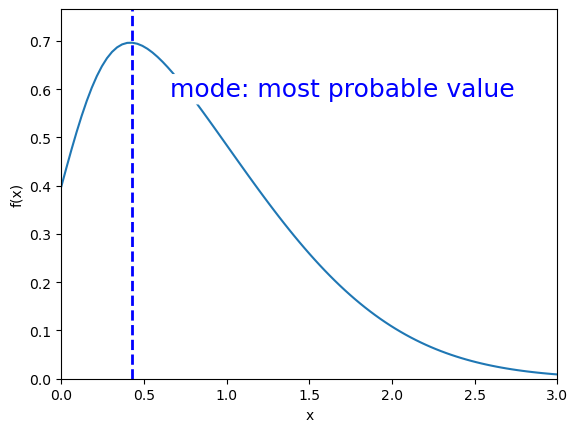
\includegraphics[scale=0.3]{PLOTDAT1-mode.png}
%%\end{center}
%
%\begin{minted}[fontsize=\small, bgcolor=LightGray]{python}
%from scipy import stats
%\end{minted}
%
%\end{frame}


\begin{frame}{Thanks For Your Time}
\center
\Huge
Fin.
\end{frame}


%\begin{frame}{Practical Reason for Normalising a function}
%I suspect my data looks like $f_X = x^3$. To check this, I need to compare \textbf{the shape} of my data distribution to \textbf{the shape} of $f_X = x^3$.\\
%I can do this if both my data histogram and my function are Normalised.\\
%To normalise the data I can just pass \texttt{density=True} as a \texttt{matplotlib} histogram argument\\
%To normalise the function I need to find a coefficient (a number) $A$ such that its integral over the range is equal to 1.\\
%
%$f_X = Ax^3$\\
%$\int_{0}^{100} f_X dx = A\int_{0}^{100}x^3 dx = A\left[\dfrac{x^4}{4}\right]_0^100 = A\left[\dfrac{(100^4-0)}{4}\right]$\\
%
%Rearranging for our normalisation coefficient $A = \dfrac{4}{100^4} = 4\times10^{-8}$\\[1ex]
%
%So $Ax^3$ normalised in the range x:[0,100] is  $(4\times10^{-8})x^3$\\
%
%
%\end{frame}



\end{document} 